\section{GOES-O(14) Sounder SRF plots}
%=====================================
\label{app:sndr_g14}
\begin{figure}[htp]
  \centering
  \begin{tabular}{c c}
    \includegraphics[scale=0.5]{graphics/nominal/sndr_g14.ch1.srf.eps} &
    \includegraphics[scale=0.5]{graphics/nominal/sndr_g14.ch2.srf.eps} \\
    \includegraphics[scale=0.5]{graphics/nominal/sndr_g14.ch3.srf.eps} &
    \includegraphics[scale=0.5]{graphics/nominal/sndr_g14.ch4.srf.eps} \\
    \includegraphics[scale=0.5]{graphics/nominal/sndr_g14.ch5.srf.eps} &
    \includegraphics[scale=0.5]{graphics/nominal/sndr_g14.ch6.srf.eps}
  \end{tabular}
  \caption{GOES-O(14) Sounder SRF for channels 1 to 6.}
  \label{fig:sndr_g14.ch1-6}
\end{figure}

\begin{figure}[htp]
  \centering
  \begin{tabular}{c c}
    \includegraphics[scale=0.5]{graphics/nominal/sndr_g14.ch7.srf.eps} &
    \includegraphics[scale=0.5]{graphics/nominal/sndr_g14.ch8.srf.eps} \\
    \includegraphics[scale=0.5]{graphics/nominal/sndr_g14.ch9.srf.eps} &
    \includegraphics[scale=0.5]{graphics/nominal/sndr_g14.ch10.srf.eps} \\
    \includegraphics[scale=0.5]{graphics/nominal/sndr_g14.ch11.srf.eps} &
    \includegraphics[scale=0.5]{graphics/nominal/sndr_g14.ch12.srf.eps}
  \end{tabular}
  \caption{GOES-O(14) Sounder SRF for channels 7 to 12.}
  \label{fig:sndr_g14.ch7-12}
\end{figure}

\begin{figure}[htp]
  \centering
  \begin{tabular}{c c}
    \includegraphics[scale=0.5]{graphics/nominal/sndr_g14.ch13.srf.eps} &
    \includegraphics[scale=0.5]{graphics/nominal/sndr_g14.ch14.srf.eps} \\
    \includegraphics[scale=0.5]{graphics/nominal/sndr_g14.ch15.srf.eps} &
    \includegraphics[scale=0.5]{graphics/nominal/sndr_g14.ch16.srf.eps} \\
    \includegraphics[scale=0.5]{graphics/nominal/sndr_g14.ch17.srf.eps} &
    \includegraphics[scale=0.5]{graphics/nominal/sndr_g14.ch18.srf.eps}
  \end{tabular}
  \caption{GOES-O(14) Sounder SRF for channels 13 to 18.}
  \label{fig:sndr_g14.ch13-18}
\end{figure}
